%!TEX root =../mapp-challenge-18-game-book.tex
% ^ leave for LaTeXTools build functionality

\phChapterWorksheet{The Kantor Region}{Opening Puzzle}

The \mappMobimon{} Expert, Dr. Treename, has gifted you with your very
first \mappMobimon{} and sent you on a journey across the
\textbf{Kantor Region} to discover new \mappMobimon{} and battle other
trainers! Kind of odd for a grown man to be sending other people's kids off
on adventures before they've even graduated high school, but hey, at least he
gave you a \textbf{Road Map}!

While visiting all twenty numbered \textbf{locations} on the map would be
great, you're a busy trainer! Upon the advice of Dr. Treename, you can
\textbf{skip out on visiting sixteen of them}.
Each of the following sixteen clues describes a different skippable location.

\begin{multicols}{2}
  \begin{itemize}
    \item Road leading W ends at location directly S. %11
    \item Its integer factors less than itself add to itself. %6
    \item Locations directly N add to \(10\). %16
    \item Exactly two neighbors, summing to \(18\). %1
    \item Flying SE would cross road connecting 8\&12. %5
    \item Roads leading N/S/E/W end at locations directly N/S/E/W. %12
    \item Odd number with five neighbors. %13
    \item N-most location with no locations directly S. %20
    \item Exactly \(3\) locations directly E. %18
    \item Has \(3\) roads leading N/S/W, each connecting to exactly one neighbor. %2
    \item Locations directly N and directly W multiply to \(11\). %14
    \item Even number with five neighbors. %10
    \item Largest prime numbered location (only factors are \(1\) and itself). %19
    \item Squared number \(x^2\) that neighbors a cubed number \(y^3\). %9
    \item Neighboring locations multiply to \(15\). %4
    \item Exactly \(4\) locations directly SW. %17
    % \item Other locations exist N/S, but not E/W. %3
    % \item Neighboring locations subtract to \(14\). %7
    % \item Exactly \(2\) even numbers N and exactly \(1\) even number W. %8
    % \item S-most location with no locations positioned N. %15
  \end{itemize}
\end{multicols}

In the above clues, a \textbf{neighbor} is a location that can be
directly accessed along a road without visiting another location first, and the
\textbf{cardinal directions} north (N), south (S), east (E), and west (W) ignore
roads unless specified.

What are the \textbf{four remaining locations}?
\textbf{Game Control} will tell you how to use this information to
solve this puzzle. Good luck!



\phWorksheet{Road Map}

\begin{center}
  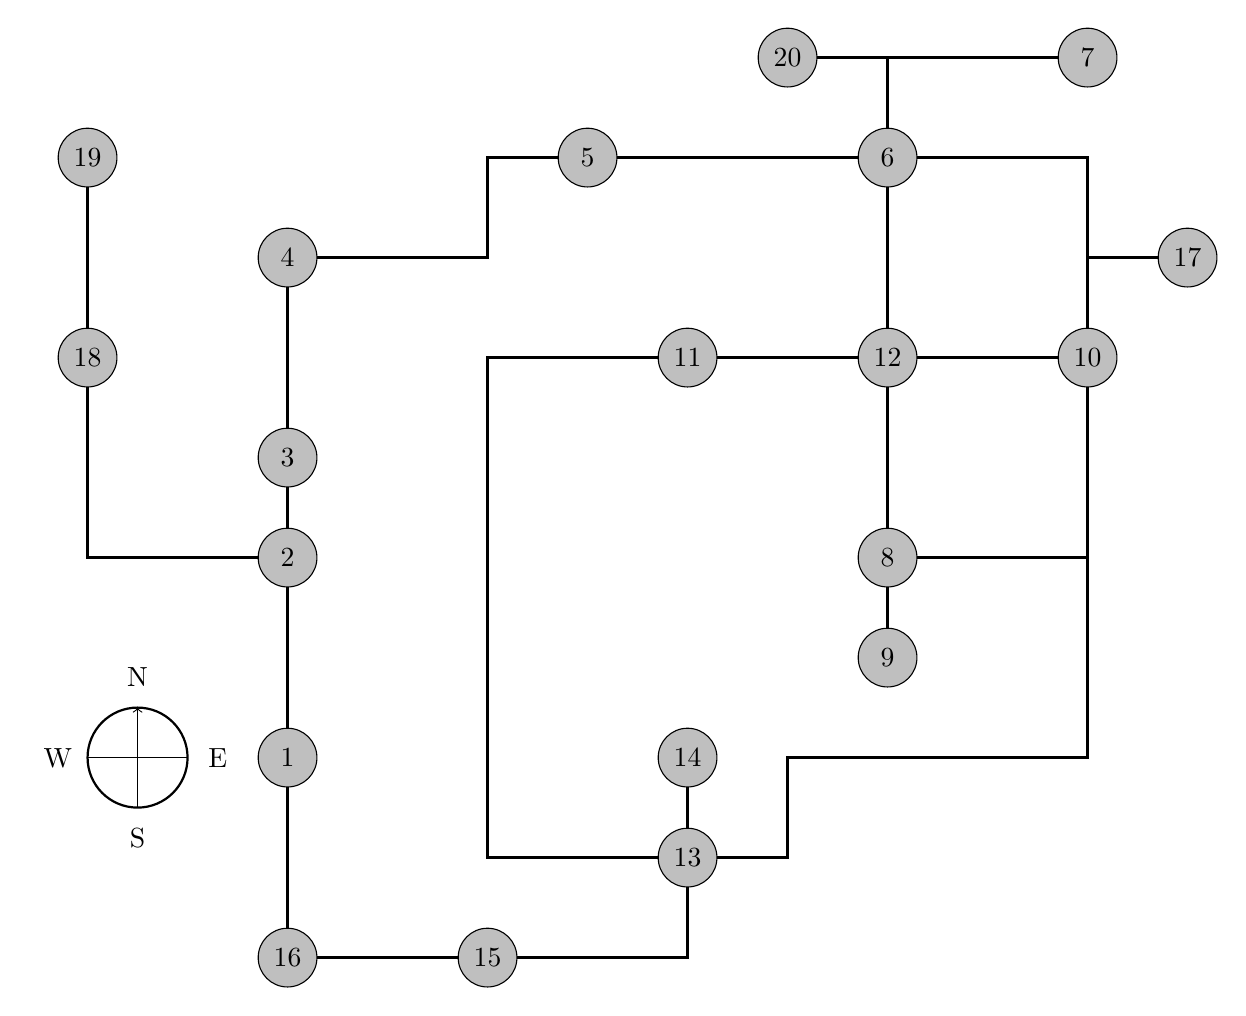
\begin{tikzpicture}[x=0.5in,y=0.5in,every node/.style={circle,fill=lightgray,
                      draw=black,text width=1em,align=center}]
    \draw[thick] (2,0) -- (2,7) -- (4,7) -- (4,8) -- (10,8) --
          (10,2) -- (7,2) -- (7,1) -- (6,1) -- (6,0) -- (2,0);
    \draw[thick] (8,9) -- (8,3);
    \draw[thick] (8,4) -- (10,4);
    \draw[thick] (7,9) -- (10,9);
    \draw[thick] (10,6) -- (4,6) -- (4,1) -- (6,1);
    \draw[thick] (10,7) -- (11,7);
    \draw[thick] (2,4) -- (0,4) -- (0,8);
    \draw[thick] (6,1) -- (6,2);

    \node at (2,2) {1};
    \node at (2,4) {2};
    \node at (2,5) {3};
    \node at (2,7) {4};
    \node at (5,8) {5};
    \node at (8,8) {6};
    \node at (10,9) {7};
    \node at (8,4) {8};
    \node at (8,3) {9};
    \node at (10,6) {10};
    \node at (6,6) {11};
    \node at (8,6) {12};
    \node at (6,1) {13};
    \node at (6,2) {14};
    \node at (4,0) {15};
    \node at (2,0) {16};
    \node at (11,7) {17};
    \node at (0,6) {18};
    \node at (0,8) {19};
    \node at (7,9) {20};

    \draw[thick] (0.5,2) circle (0.5);
    \draw (0,2) -- (1,2);
    \draw[->] (0.5,1.5) -- (0.5,2.5);
    \node[draw=none,fill=none,anchor=south] at (0.5,2.5) {N};
    \node[draw=none,fill=none,anchor=north] at (0.5,1.5) {S};
    \node[draw=none,fill=none,anchor=west] at (1,2) {E};
    \node[draw=none,fill=none,anchor=east] at (0,2) {W};
  \end{tikzpicture}
\end{center}

% Include below for aucTeX integration
%%% Local Variables:
%%% mode: latex
%%% TeX-master: "../mapp-challenge-18-game-book"
%%% End:
